\begin{mdframed}[frametitle={Change in notation}, nobreak=false]
    From this section onward, $\Omega$ (`Omega') denotes the frequency in the context of a continuous-time signal; whereas $\omega$ (`omega') denotes the frequency in the context of a discrete-time signal. \\

    Hence, the continuous-time Fourier transform (CTFT):
    \[
        \underbrace{X(\omega) = \int_{-\infty}^{+\infty} x(t) e^{-j\omega t} \mathrm{d}t}_{\text{old notation}}
        \quad \Rightarrow \quad 
        \underbrace{X(j\Omega) = \int_{-\infty}^{+\infty} x(t) e^{-j\Omega t} \mathrm{d}t}_{\text{new notation}}
    \]
\end{mdframed}


\section{Sampling}
\begin{figure}[H]
    \centering
    \begin{tikzpicture}[auto, node distance=2.2cm,>=Latex]
        % Nodes
        \node (input) {$x_c(t)$};
        \node [draw, rectangle, minimum width=2cm, minimum height=1cm, right=.7cm of input] (block1) {\textbf{C/D converter}};
        \node [right=.35cm of block1] (xn) {};
        \node [below=0.05cm of xn] (xn_label) {$x[n]$};
        \node [draw, rectangle, minimum width=2cm, minimum height=1cm, right=.35cm of xn] (block2) {\textbf{discrete-time system}};
        \node [right=.35cm of block2] (yn) {};
        \node [below=0.05cm of yn] (yn_label) {$y[n]$};
        \node [draw, rectangle, minimum width=2cm, minimum height=1cm, right=.35cm of yn] (block3) {\textbf{D/C converter}};
        \node [right=0.7cm of block3] (output) {$\hat{y}_r(t)$};
    
        \node[below=0.5cm of block1](T1){$T$};
        \node[below=0.5cm of block3](T3){$T$};
        
        % Arrows
        \draw[->] (input) -- (block1);
        \draw[->] (block1) -- (block2);
        \draw[->] (block2) -- (block3);
        \draw[->] (block3) -- (output);
        \draw[->] (T1) -- (block1);
        \draw[->] (T3) -- (block3);
    
        % Labels below arrows
        \node [below=0.1cm of input] {};
        \node [below=0.1cm of xn] {};
        \node [below=0.1cm of yn] {};
    \end{tikzpicture}
    \caption{A very-brief overview of  digital processing of continuous-time signals}
    \label{fig:dsp_short}
\end{figure}
\autoref{fig:dsp_short} illustrates a concise process of digital processing of a continuous-time signal. 
\begin{itemize}
    \item The C/D conversion involves sampling a continuous-time signal to obtain a discrete-time signal.

    \item The D/C conversion involves the reconstruction of a continuous-time signal from the sampled discrete-time signal.
\end{itemize} 

\subsection{Sampling of a Continuous-Time Signal}
Mathematically, sampling of a continuous-time signal $x_{c}(t) \to x[n]$ is:
\[ x[n] = x_{c}(nT) \quad \text{for} \ -\infty < n < +\infty \]
where $T$ is sampling period, $f_{s} = \dfrac{1}{T}$ is sampling frequency (or $\Omega_{s}=\dfrac{2\pi}{T}$ in radians). 
\begin{itemize}
    \item In general, the C/D transformation cannot be inverted.
    \item Infinite continuous signals can reproduce a given sequence of samples,
\end{itemize}
An ideal C/D converter applies the $T$ property so that the sampling can be done without losing information. \\


Impulse train modulator $s(t)$ is: 
\[ 
    s(t) = \sum_{n=-\infty}^{+\infty} \ \delta(t-nT) 
\]
The sampled signal $x_{s}(t)$ is obtained by multiplying the impulse train modulator (\autoref{fig:original_signal}.b) with the continuous-time signal $x_{c}(t)$ of interest (\autoref{fig:original_signal}.a):
\begin{align*} 
\begin{split}
x_{s}(t) &= x_{c}(t) \ s(t)\\
&= \sum_{n=-\infty}^{+\infty} x_{c}(t) \delta(t-nT)\\
&= \sum_{n=-\infty}^{+\infty} x_{c}(nT) \delta(t-nT)
\end{split}
\end{align*}
The sampled signal, $x_{s}(t)$, is still defined in the continuous-time domain, but it contains all information in the sampled discrete-time domain.\\

Apply the Fourier transform ($\mathcal{F}\{\cdot\}$) to $x_{s}(t)$:
\begin{align*} 
\begin{split}
    X_{s}(\Omega) 
    & = \mathcal{F}\{x_{c}(t)\} \cdot \mathcal{F}\{s(t)\}\\
    & = \frac{1}{2\pi} X_{c}(\Omega) * \mathcal{F}\{s(t)\} \\
    & = \frac{1}{T} X_{c}(\Omega) * \sum_{n=-\infty}^{+\infty} \delta (\Omega - k \Omega_{s})\\
    & = \boxed{\frac{1}{T} \sum_{n=-\infty}^{+\infty}  X_{c}(\Omega - k \Omega_{s})}
\end{split} 
\end{align*}
where sampling frequency $\Omega_{s}=\Omega_{0}=\frac{2\pi}{T}$.

\begin{figure}[H]
\centering
    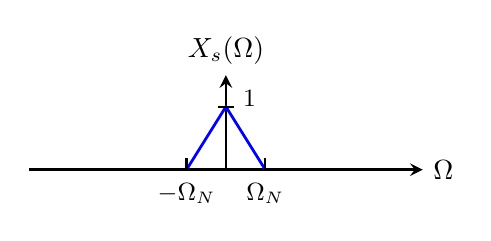
\begin{tikzpicture}
        \centering 
        % Set up styles
        \tikzset{line style/.style={thick}}
        % Frequency axis
        \draw[-stealth, line width=1pt] (-2.5, 0) -- (2.5, 0) node[right] {$\Omega$};
        \draw[-stealth, line width=1pt] (0, 0) -- (0, 1.2) node[above] {$X_{s}(\Omega)$};
        % Draw and label the triangles
        \draw[line style, line width=1pt, blue] (-0.5, 0) -- (0, 0.8) -- (0.5, 0);
        \draw[line style] (0, 0) -- (0, 0.15);
        \draw[line style] (0.5, 0) -- (0.5, 0.15);
        \draw[line style] (-0.5, 0) -- (-0.5, 0.15);
        % Label the frequency points
        \node at (0.5, -0.3) {\small$\Omega_N$};
        \node at (-0.5, -0.3) {\small$-\Omega_N$};
        % peak value
        \draw[line style] (-0.1, 0.8) -- (0.1, 0.8);
        \node at (0.3, 0.9) {\small 1};
    \end{tikzpicture}
    \hspace{.1\textwidth}
    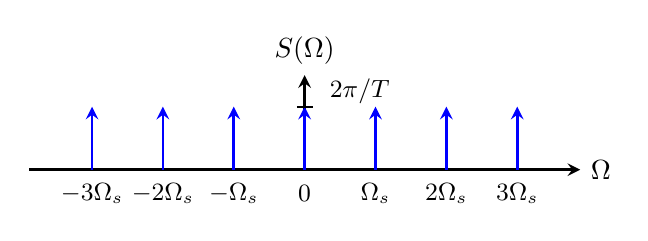
\begin{tikzpicture}
        \tikzset{line style/.style={thick}}
        % Frequency axis
        \draw[-stealth, line width=1pt] (-3.5, 0) -- (3.5, 0) node[right] {$\Omega$};
        \draw[-stealth, line width=1pt] (0, 0) -- (0, 1.2) node[above] {$S(\Omega)$};
        % Draw and label the main triangles and dashed extensions
        \foreach \x in {-2.7, -1.8, -0.9, 0, 0.9, 1.8, 2.7} {
            \draw[line style, -stealth, blue, line width=1pt] (\x, 0) -- (\x, 0.8);
        }
        \node at (-0.9, -0.3) {\small$-\Omega_s$};
        \node at (-1.8, -0.3) {\small$-2\Omega_s$};
        \node at (-2.7, -0.3) {\small$-3\Omega_s$};
        \node at (0, -0.3) {\small 0};
        \node at (0.9, -0.3) {\small$\Omega_s$};
        \node at (1.8, -0.3) {\small$2\Omega_s$};
        \node at (2.7, -0.3) {\small$3\Omega_s$};
        % peak
        \draw[line style] (-0.1, 0.8) -- (0.1, 0.8);
        \node at (0.7, 1) {\small$2\pi/T$};
    \end{tikzpicture}
    \caption{Spectrum of (left) the original continuous-time signal to be sampled, $X_s(\Omega)$ and (right) the sampler $S(\Omega)$ (as a $\delta$-train).}
    \label{fig:original_signal}
\end{figure}

For sampled signals: $\Omega_{N}$ is the signal bandwidth
\begin{itemize}
    \item if $\Omega_{s} \geq 2\Omega_{N}$, the replicas in the periodization do not overlap (\autoref{fig:aliasing}.a)
    \item if $\Omega_{s} < 2\Omega_{N}$, the replicas overlap, also known as \textbf{aliasing}(\autoref{fig:aliasing}.b).
\end{itemize} 

\begin{figure}[H]
%% first figure
\begin{subfigure}{.45\textwidth}
\centering
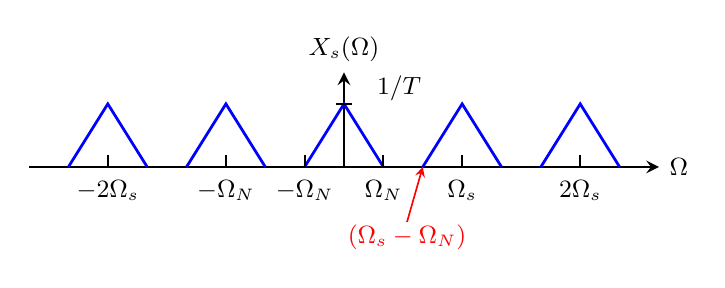
\begin{tikzpicture}
    \tikzset{line style/.style={thick}}
    % frequency axis
    \draw[-stealth, line width=1pt] (-4, 0) -- (4, 0) node[right] {\small$\Omega$};
    \draw[-stealth, line width=1pt] (0, 0) -- (0, 1.2) node[above] {\small $X_{s}(\Omega)$};

    % draw and label the triangles
    \foreach \x in {-3, -1.5, 0, 1.5, 3} {
        \draw[line style, line width=1pt, blue] (\x-0.5, 0) -- (\x, 0.8) -- (\x+0.5, 0);
        \draw[line style] (\x, 0) -- (\x, 0.15);
    }
    \draw[line style] (0.5, 0) -- (0.5, 0.15);
    \draw[line style] (-0.5, 0) -- (-0.5, 0.15);
    
    % label the frequency points
    \node at (0.5, -0.3) {\small$\Omega_N$};
    \node at (-0.5, -0.3) {\small$-\Omega_N$};
    \node at (1.5, -0.3) {\small$\Omega_s$};
    \node at (-1.5, -0.3) {\small$-\Omega_N$};
    \node at (3, -0.3) {\small$2\Omega_s$};
    \node at (-3, -0.3) {\small$-2\Omega_s$};

    % peak value
    \draw[line style] (-0.1, 0.8) -- (0.1, 0.8);
    \node at (0.7, 1) {\small$1/T$};

    % x values below the triangles
    \node[red] at (0.8, -0.9) {\small$(\Omega_s - \Omega_N)$};
    \draw[-stealth, red, line width=.6pt] (0.8, -0.7) -- (1, 0);
\end{tikzpicture}
\caption{Sampling without aliasing when $\Omega_{s} \geq 2\Omega_{N}$.}
\end{subfigure}
\hfill
%% second figure
\begin{subfigure}{.45\textwidth}
\centering
    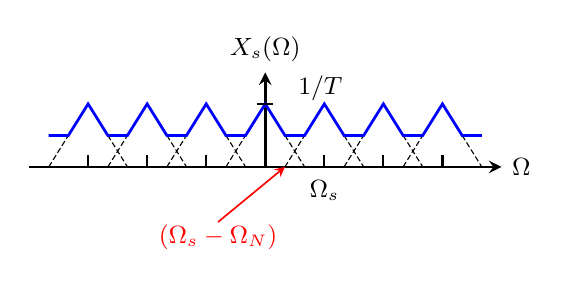
\begin{tikzpicture}
    \tikzset{line style/.style={thick}}
    \tikzset{dashed style/.style={thick, dashed}}

    % Frequency axis
    \draw[-stealth, line width=1pt] (-3, 0) -- (3, 0) node[right] {\small $\Omega$};
    \draw[-stealth, line width=1pt] (0, 0) -- (0, 1.2) node[above] {\small $X_{s}(\Omega)$};

    % Draw and label the main triangles and dashed extensions
    \foreach \x in {-2.25, -1.5, -0.75, 0, 0.75, 1.5, 2.25} {
        \draw[dash pattern=on 2pt off 1pt] (\x-0.5, 0) -- (\x-0.25, 0.4) ;
        \draw[dash pattern=on 2pt off 1pt] (\x+0.25, 0.4) -- (\x+0.5, 0) ;
        \draw[line style, line width=1pt, blue]  (\x-0.5, 0.4) -- (\x-0.25, 0.4) -- (\x, 0.8) -- (\x+0.25, 0.4) -- (\x+0.5, 0.4);
        \draw[line style] (\x, 0) -- (\x, 0.15);
    }
    \node at (0.75, -0.3) {\small$\Omega_s$};

    % peak
    \draw[line style] (-0.1, 0.8) -- (0.1, 0.8);
    \node at (0.7, 1) {\small$1/T$};
    % \node at (0.3, 1.9) {$X_s(\omega)$};

    % x values below the triangles
    \node[red] at (-0.6, -0.9) {\small$(\Omega_s - \Omega_N)$};
    \draw[-stealth, red, line width=.6pt] (-0.6, -0.7) -- (0.25, 0);
\end{tikzpicture}
\caption{Sampling with aliasing when $\Omega_{s} < 2\Omega_{N}$}
\end{subfigure}
\caption{The signal copies remain separate under a high sampling rate; while the signals are overlapped (aliasing) with a lower sampling rate.} 
\label{fig:aliasing}
\end{figure}



\subsubsection{Nyquist-Shannon Sampling Theorem}
Nyquist-Shannon sampling theorem states that: \textbf{to retain the ability to reproduce (reconstruct) the original signal, the minimum sampling frequency during signal sampling must be at least twice its frequency.}\\

Mathematically, let $x_{c}(t)$ be a band-limited signal with $X_{c}(\Omega)=0$, for $\lvert \Omega \rvert \geq \Omega_{N}$. Then $x_{c}(t)$ is uniquely determined by its samples $x[n] = x_{c}(nT)$, if 
\[ \Omega_{s}=\frac{2\pi}{T} \geq 2\Omega_{N} \]
where $2\Omega_{N}$ is the minimal sampling rate and referred to as the \textbf{Nyquist rate}.\\

Nyquist-Shannon sampling theorem provides the condition under which the C/D transformation \textbf{can be inverted} without losing information, as shown in \autoref{fig:nyquist}.

\begin{figure}[H]
    \centering
    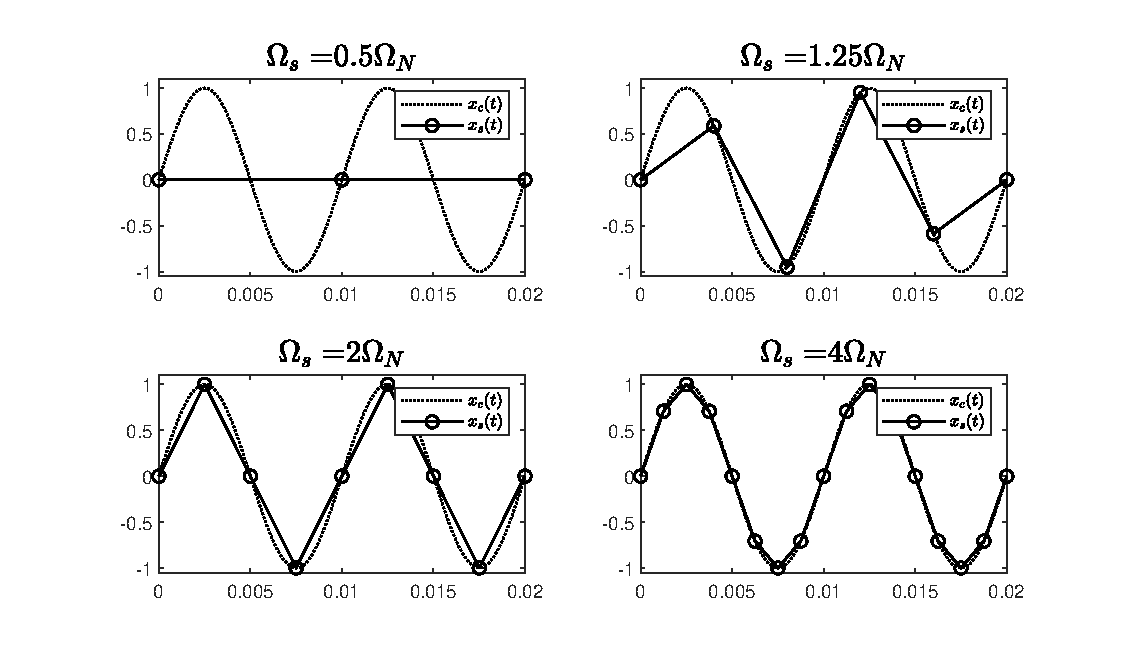
\includegraphics[width=\textwidth, center]{images/nyquist.eps}
    \caption{Sampling of a continuous signal $x_{c}(t)=\sin(200\pi t)$: (left to right, top to bottom) $\Omega_{s}=0.5\Omega_{N}$, $\Omega_{s}=1.25\Omega_{N}$, $\Omega_{s}=2\Omega_{N}$, $\Omega_{s}=4\Omega_{N}$. According to the Nyquist-Shannon sampling theorem, aliasing occurs when $\Omega_{s} < 2\Omega_{N}$}
    \label{fig:nyquist}
\end{figure}

\subsection{Practical Digital Processing of Continuous-Time Signals}
\begin{figure}[H]
    \centering
    \resizebox{\textwidth}{!}{
    \begin{tikzpicture}[auto, node distance=1cm,>=Latex]
        % Nodes
        % 1
        \node (input) {$x_c(t)$};
        \node [draw, rectangle, minimum width=2.5cm, minimum height=1cm, right=.7cm of input] (block1) {\parbox{2.5cm}{\centering \textbf{anti-aliasing filter}}};
        \node[above=.15cm of block1]{$H_{aa}(j\Omega)$};
        \node [right=.45cm of block1] (xat) {};
        \node [below=0.05cm of xat] (xat_label) {$x_{a} (t)$};
        % 2
        \node [draw, rectangle, minimum width=2cm, minimum height=1cm, right=.45cm of xat] (block2) {\parbox{2cm}{\centering \textbf{sample and hold}}};
        \node [right=.45cm of block2] (x0t) {};
        \node [below=0.05cm of x0t] (x0t_label) {$x_{0}(t)$};
        % 3
        \node [draw, rectangle, minimum width=2cm, minimum height=1cm, right=.45cm of x0t] (block3) {\parbox{2cm}{\centering \textbf{A/D converter}}};
        \node [right=.45cm of block3] (xhatn) {};
        \node [below=0.05cm of xhatn] (xhatn_label) {$\hat{x}[n]$};
        % 4
        \node [draw, rectangle, minimum width=2.5cm, minimum height=1cm, right=.45cm of xhatn] (block4) {\parbox{2.5cm}{\centering \textbf{discrete-time system}}};
        \node [right=.45cm of block4] (yhatn) {};
        \node [below=0.05cm of yhatn] (yhatn_label) {$\hat{y}[n]$};
        % 5
        \node [draw, rectangle, minimum width=2cm, minimum height=1cm, right=.45cm of yhatn] (block5) {\parbox{2cm}{\centering \textbf{D/A converter}}};
        \node [right=.45cm of block5] (yDA) {};
        \node [below=0.05cm of yDA] (yDA_label) {$y_{DA}(t)$};
        % 6
        \node [draw, rectangle, minimum width=2.7cm, minimum height=1cm, right=.45cm of yDA] (block6) {\parbox{2.7cm}{\centering \textbf{reconstruction filter}}};
        \node[above=.15cm of block6]{$H_{aa}(j\Omega)$};
        \node [right=0.7cm of block6] (output) {$\hat{y}_{r}(t)$};
        % T symbs
        \node[below=0.5cm of block2](T2){$T$};
        \node[below=0.5cm of block3](T3){$T$};
        \node[below=0.5cm of block5](T5){$T$};
        
        % Arrows
        \draw[->] (input) -- (block1);
        \draw[->] (block1) -- (block2);
        \draw[->] (block2) -- (block3);
        \draw[->] (block3) -- (block4);
        \draw[->] (block4) -- (block5);
        \draw[->] (block5) -- (block6);
        \draw[->] (block6) -- (output);
        \draw[->] (T2) -- (block2);
        \draw[->] (T3) -- (block3);
        \draw[->] (T5) -- (block5);
    \end{tikzpicture}
    }
    \caption{Overview of practical digital processing of continuous-time signals}
    \label{fig:dsp}
\end{figure}

\paragraph{Ideal anti-aliasing filter: $x_{c}(t) \to x_{a}(t)$}
\[
    H_{aa}(j\Omega) = 
    \begin{cases}
    1,  & \lvert \Omega \rvert \leq \pi/T \\
    0,  & \lvert \Omega \rvert > \pi/T
    \end{cases}
\]

\paragraph{Sample and hold: $x_{a}(t) \to x_{0}(t)$}
\[
    x_0(t) = h_0(t) * \sum_{n=-\infty}^{\infty} x_{c}(nT)\delta(t-nT)
\]

\paragraph{Practical D/A conversion: $\hat{y}[n] \to y_{DA}(t)$}
\[
    x_{c}(t) = \sum_{n=-\infty}^{+\infty} x_{c}(nT)h_{r}(t-nT) = \sum_{n=-\infty}^{+\infty} x_{c}(nT) \frac{\sin(\pi(t-nT)/T)}{\pi(t-nT)/T}
\]
\[
    x_{DA}(t) = \sum_{n=-\infty}^{+\infty} x[n]h_{p}(t-nT) + \sum_{n=-\infty}^{+\infty} e[n]h_{p}(t-nT)
\]

\subsection{Example Questions}
\begin{q}{}
The continuous-time signal $x_{c}(t)$ is sampled with sampling frequency $\Omega_{s}$ to obtain the sampled signal $x_{s}(t) = x_{c}(t) \sum_{-\infty}^{+\infty} \delta(t-nT)$ with $T$ being the sampling interval ($\Omega_s = \frac{2\pi}{T}$). The Fourier transform of $x_{c}(t)$ is $X_{c}(j\Omega) = \frac{1}{\Omega_{N}} \lvert \Omega \rvert + 1$ for $\lvert \Omega \rvert \leq \Omega_N$ and $X_{c}(j\Omega) = 0$ for $\lvert \Omega \rvert > \Omega_N$. Assuming $\Omega_{s} = \Omega_{N}$, which of the following expressions for the sampled signal $x_{s}(t)$ is correct? 

\begin{enumerate}[label=(\alph*)]
    \item $x_{s}(t) = x_{c}(t)$
    \item $x_{s}(t) = \frac{1}{T}\delta(t)$
    \item $x_{s}(t) = \sum_{-\infty}^{+\infty} \delta(t-nT)$
    \item $x_{s}(t) = 0$
    \item $x_{s}(t) = \sum_{-\infty}^{+\infty} x_{c}(t-nT)$
\end{enumerate}

\paragraph{Answer}

\end{q}
%==============================================%

